\chapter{Flux calibration}
\label{sec:flux}

\section{How \banzai{} selects and uses standards}
\label{sec:flux_banzai}
\banzai{} selects the flux standard in this order: the same observing block; otherwise the closest in time from the
same proposal; otherwise any public standard. Standards are \emph{not} matched by slit width. The Fairall~9 frames
therefore used the eight 6\,arcsec standards taken by the RM proposal between 2026 September 22 and October 8, and
every frame after October 8 used the October 8 standard, although a 2\,arcsec EG\,21 spectrum from LCO's standards
programme exists on most nights. EG\,21 is, moreover, absent from \banzai's flux-standard catalogue (which lists
GD\,108, EG\,274, Feige\,110, Feige\,34 and BD$+28^\circ4211$), so the 18 EG\,21 observations never produced a
sensitivity function and were themselves calibrated with the October 8 standard. The red-order sensitivity of the
October 3 standard has a spike ($+20/-5$ in $\ln S$) at 5200\,\AA. In 1.0.1 the sensitivity is a B-spline in $\ln S$
with fine knots, which also follows the fringes of the standard (Fig.~\ref{fig:sens}).

\textit{Absolute level of the archive spectra.} The archive Fairall~9 spectra are $2.2\pm0.3$ times brighter than
the same exposures reduced with \banzai{}~1.1.0 (stock) or with improved v3, at all wavelengths and for all epochs (also for the
33 epochs calibrated with the same October 8 standard), while the extracted counts agree to 1--4 per cent and EG\,21
agrees with its reference in all reductions. The cause is the exposure time: in 1.0.1 the sensitivity is the
expected flux of the standard over its \emph{counts}, and \texttt{flux\_calibrate} multiplies the science counts by
it without dividing by any exposure time, so a science frame is scaled by $t_{\rm sci}/t_{\rm std}$ = 600\,s/300\,s
= 2 for Fairall~9 (the remaining $\approx10$ per cent is the 1.0.1 sensitivity itself, a Savitzky--Golay filter of
expected over observed counts). EG\,21 (300\,s, like the standards) is unaffected. 1.1.0 uses count rates, and the
improved v3 agrees with \banzai{}~1.1.0 (stock) to 4 per cent. In the raw headers the October 8 standard
(\texttt{coj2m002-en12-20261008-0001}) is Feige\,110 through the 2\,arcsec slit. Since all the
standards of the campaign are 2\,arcsec while Fairall~9 is observed through 6\,arcsec, the absolute level of the
final spectra is still biased high by the slit losses of the standards (seeing-dependent; the grey normalisation to
the clearest standards, which have the lowest $S$, keeps the bias at its minimum); RM light curves, which are
scaled to [O\,{\sc iii}], are not affected.

\begin{figure}[!htbp]
\centering
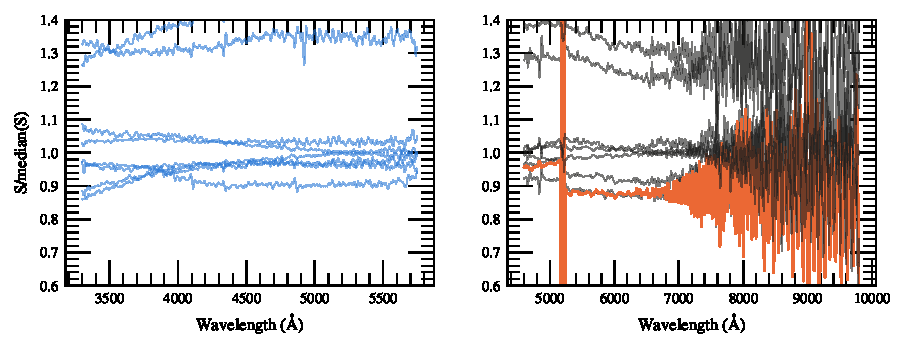
\includegraphics[width=\textwidth]{figures/fig_sens.pdf}
\caption{The eight sensitivity functions used by the archive Fairall~9 spectra, each divided by their median. Orange:
the 2026-10-03 standard (spike at 5200\,\AA). Redward of 7000\,\AA{} the fine-knot fit has learned the fringes of
each standard.}
\label{fig:sens}
\end{figure}


\section{Template $\times$ nightly correction}
\label{sec:flux_model}
Many standards, including EG\,21, have only low-resolution reference fluxes (here the CTIO spectrum in 50\,\AA{} bins;
\citealt{Hamuy1992,Hamuy1994}), which cannot resolve the instrumental notches of the blue order (50--150\,\AA{} wide).
We therefore write the sensitivity of night $n$ and order $o$ as
\begin{equation}
S_{n,o}(\lambda)=T_o(\lambda)\,\exp\left[\sum_{k=0}^{4}p_{n,o,k}\,L_k(\tilde\lambda)\right],
\label{eq:sens}
\end{equation}
where the template $T_o$ carries the fine structure and the Legendre series the smooth, night-dependent part. $T_{\rm
blue}$ is the median of the eight 6\,arcsec sensitivities of \banzai{} (each grey-normalised); $T_{\rm red}$ is the
median of the six good ones smoothed with a 401\,\AA{} running median (no fine structure is needed in the red once
the fringes are removed in the extraction). With $C(\lambda)$ the count rate of the standard corrected for
extinction,
\begin{equation}
C(\lambda)=\frac{N(\lambda)}{t_{\rm exp}\,\tau(\lambda,X)},
\label{eq:rate}
\end{equation}
\begin{equation}
\tau(\lambda,X)=\left[10^{-0.4\,k(\lambda)}\right]^{X\exp[-(h-2788\,{\rm m})/10\,400\,{\rm m}]},
\label{eq:ext}
\end{equation}
($k$ the APO extinction curve shipped with \banzai, $h=1149$\,m for COJ), the coefficients $p_{n,o,k}$ are fitted
to
\begin{equation}
y_j=\ln\frac{F^{\rm ref}_j}{\langle C\,T_o\rangle_j}
\label{eq:sensfit}
\end{equation}
in the reference bins $j$ ($\langle\cdot\rangle_j$ the mean over the bin, required to be $\ge80$ per cent populated),
excluding bins overlapping telluric bands or the cores ($\pm40$\,\AA) of the Balmer lines, with iterative $3\sigma$
clipping.

\textit{Quality control and grey level.} For each order the fitted $P_n(\lambda)$, after removing its median, is compared
with the median over all standards on a grid; a standard deviating by more than $4\times\max(\mathrm{MAD}\times1.4826,
0.02)$ anywhere is rejected. Clouds during the standard exposure raise $S=F^{\rm ref}/C$ grey-ly; to keep the nightly
shape without transferring the standard's clouds, each standard's sensitivity (both orders) is multiplied by
$\exp(\bar g-g_n)$, with $g_n$ the median of $\ln S_{n,{\rm red}}$ at 5500--6500\,\AA{} and $\bar g$ the median of $g_n$
over the clearest (lowest-$g$) half of the standards.

\section{Ensemble flux calibration in the pipeline}
\label{sec:flux_ensemble}
In the reduction from raw the grey normalisation and the ensemble are part of \texttt{FluxCalibrator}
(\texttt{FLUX\_ENSEMBLE\_DAYS}, \texttt{FLUX\_ENSEMBLE\_N}). Each standard still gets its own sensitivity from the
1.1.0 stage \texttt{FluxSensitivity} (a B-spline in $\ln S$ with knots every 20\,\AA{} blueward of 6500\,\AA{} and
every 600\,\AA{} redward, fitted after the harmonic fringe correction). A science frame then uses, instead of the
sensitivity of the single nearest standard, the median of the sensitivities of the nine standards nearest in time
(within $\pm90$\,d), each first multiplied by $\exp(\bar g-g_n)$ as above, with $\bar g$ the median level of the
clearest half of those nine (\texttt{FLUX\_GREY\_WINDOW}, \texttt{FLUX\_GREY\_CLEAR\_FRACTION}). The same nine
standards provide the telluric transmission (Section~\ref{sec:flux_tell}). The grey levels of nine consecutive
Feige\,110 exposures typically span a factor of two, i.e.\ clouds during the 300\,s standard were otherwise
transferred to the science. The template of eq.~\ref{eq:sens} is not needed with Feige\,110, whose reference is
sampled every 2\,\AA; it remains the method for standards with coarse references such as EG\,21. The frame header
records the number of standards and the spread of their grey factors (\texttt{L1FLXNST}, \texttt{L1FLXGRY}).

\section{Telluric correction and application}
\label{sec:flux_tell}
The telluric transmission is measured on the same standard: the calibrated standard $C\,S$ is fitted outside the
bands with a smoothing spline $\mathcal{C}(\lambda)$ in $\ln$, and $t(\lambda)=C\,S/\mathcal{C}$ inside the bands
(clipped to $[0.02,1]$; $t=1$ outside). A science frame at airmass $X_{\rm s}$ calibrated with a standard at $X_\star$
is then
\begin{equation}
F_\lambda=\frac{N(\lambda)\,S(\lambda)}{t_{\rm exp}\,\tau(\lambda,X_{\rm s})\,t(\lambda)^{X_{\rm s}/X_\star}},
\label{eq:apply}
\end{equation}
By default $S$ and $t$ are the medians over all good standards of $S_n$ (grey-normalised) and of $t_n^{1/X_{\star,n}}$
(then raised to $X_{\rm s}$); the standard closest in time can be used instead. The median transfers better between
nights (Section~\ref{sec:results_flux}): the smooth part of a single 2\,arcsec standard partly reflects that night's
slit losses, which do not apply to another night or to a 6\,arcsec spectrum. Because RM inter-calibration removes
grey factors, all comparisons below are made on spectral \emph{shapes} unless stated otherwise.


\textit{The telluric model in the pipeline.} \banzai{}~1.1.0 measures the transmission on the standard in broad
regions that together cover almost the whole red order (6400--7500, 7800--8690 and 8730--9960\,\AA) and divides
every science spectrum by it. Outside the real absorption bands this ratio is the standard's noise and residual
structure: its 12/150\,\AA{} high-pass has an rms of 0.9--1.1 per cent at 6960--8050\,\AA{} and 3 per cent at
8450--8900\,\AA, and it reappears unchanged in every science spectrum, where it was the main remaining source of
fringe-like bumps at 6500--7500\,\AA{} after the harmonic fringe correction. Applying the transmission only in the
absorption bands (\texttt{TELLURIC\_MODEL\_BANDS}) lowers the high-pass rms of the Fairall~9 spectra from 3.4 to 3.0 per cent at
6400--6850\,\AA{} and from 4.3 to 3.4 per cent at 8450--8900\,\AA. For a science frame taken through the same slit as
the standard (EG\,21 with the 2\,arcsec Feige\,110 standards) the broad division is slightly better (0.9 against
1.0 per cent at 6960--7150\,\AA), because part of the residual structure belongs to the slit configuration and
cancels; for 6\,arcsec RM spectra calibrated with 2\,arcsec standards it does not.
The bands are where the Matheson et al.\ (2000) transmission at 9\,\AA{} resolution is more than 1 per cent below
unity: 6850--7090 (O$_2$ B band), 7135--7400 (H$_2$O), 7560--7720 (O$_2$ A band), 7870--8050 and 8085--8400
(H$_2$O) and 8900--9900\,\AA. A first choice that stopped at the band cores (6860--6960, 7150--7350 and
8100--8380\,\AA) left the wings uncorrected: a 1--2 per cent deficit at 6960--7090 and 7350--7400\,\AA, conspicuous
in the flux-calibrated standards (Fig.~\ref{fig:zoom}).

\textit{The O$_2$ A band.} In the 6\,arcsec Fairall~9 spectra the saturated A band (7590--7700\,\AA) leaves a residual
common to all spectra, +25 per cent at the band head and $-17$ per cent at 7620\,\AA{} (10 per cent rms of the median
over spectra), while in EG\,21, taken through the same 2\,arcsec slit as the standards, it is 1.7 per cent
(Fig.~\ref{fig:aband}). The transmission measured through the 2\,arcsec slit resolves the band head differently
from a 6\,arcsec spectrum, and the fringes (10--12 per cent there) are interpolated across the band in both. Sky lines
cannot provide the line-spread function of the object: they fill the slit ($\sigma=35$\,\AA{} through 6\,arcsec
against 6.7\,\AA{} through 2\,arcsec). Broadening the transmission by a fixed $\sigma=5$\,\AA, or by a width fitted to
each frame's own A band or to its water band, lowers the per-spectrum residual of Fairall~9 only from 8.4 to 7.8, 6.4
(fitted on the A band itself, an optimistic bound) and 8.0 per cent. The band is therefore flagged in the science
spectra: 7580--7700\,\AA{} carries bit 2 in the \texttt{mask} column (\texttt{TELLURIC\_FLAG\_BANDS}; header
\texttt{L1TELFLG}); the flux values are kept.

\begin{figure}[!htbp]
\centering
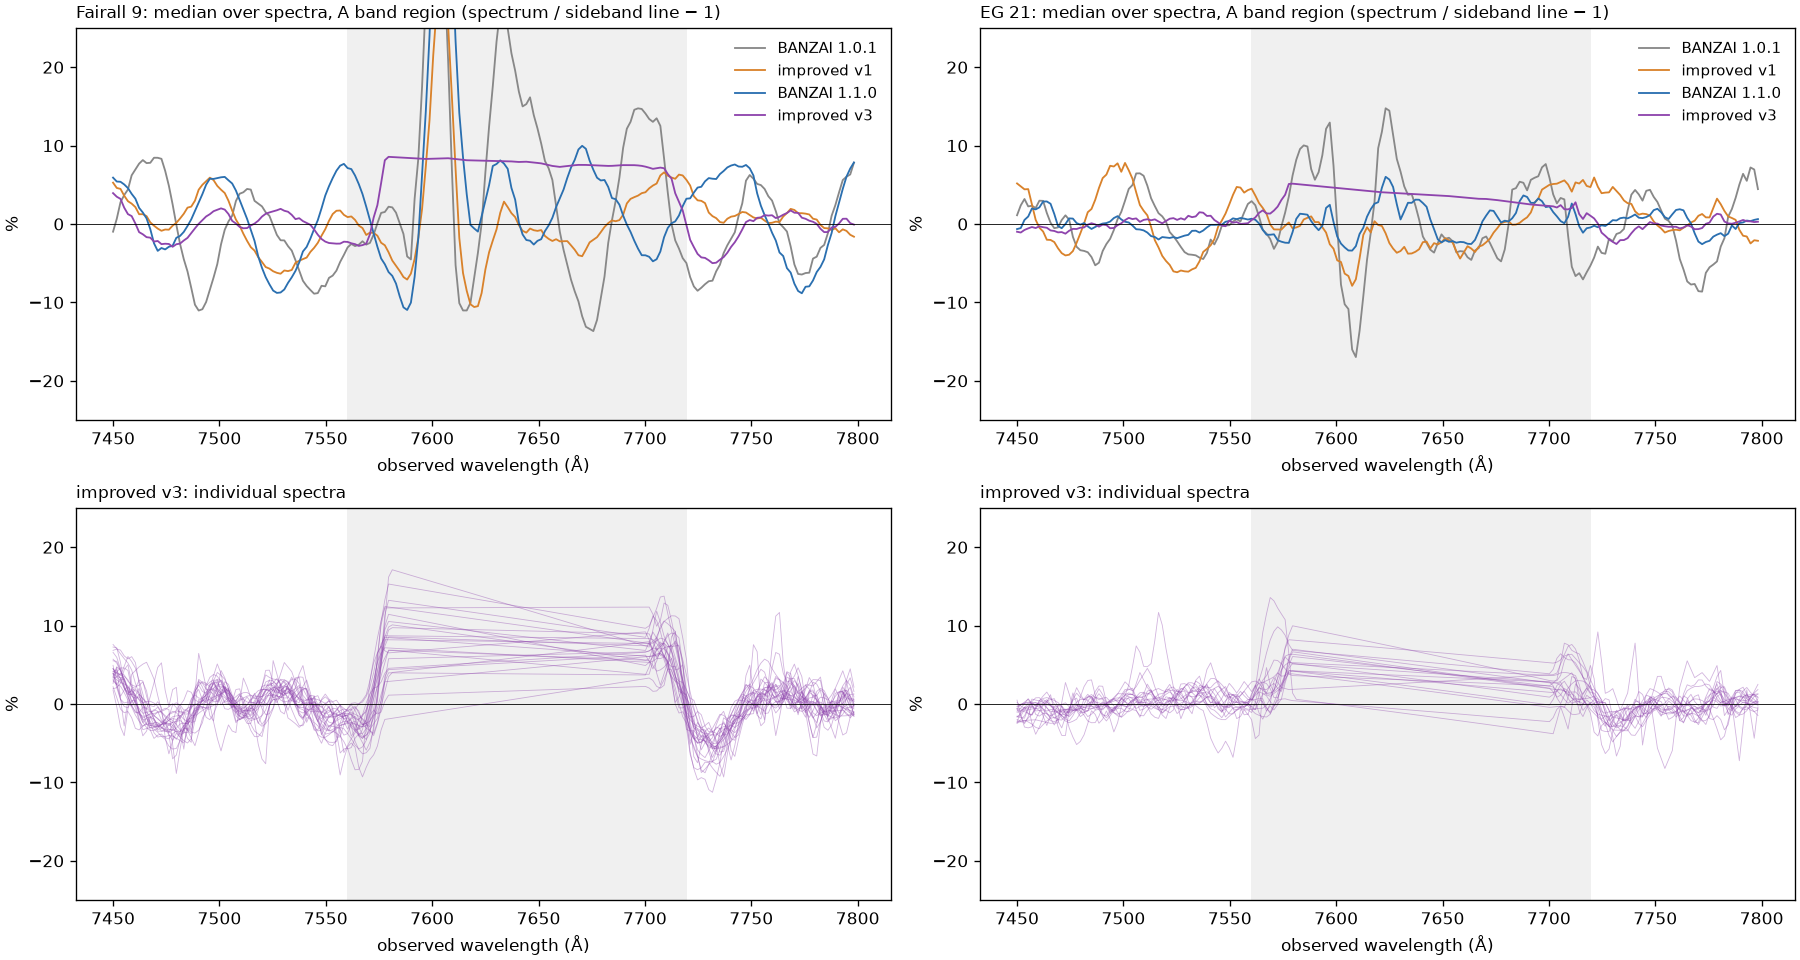
\includegraphics[width=\textwidth]{figures/fig_aband.png}
\caption{The O$_2$ A band: each spectrum over a straight line through the sidebands (7450--7545 and
7735--7800\,\AA). Top: median over spectra for the reductions; bottom: individual spectra of improved v3. Left:
Fairall~9 (6\,arcsec); right: EG\,21 (2\,arcsec, as the standards).}
\label{fig:aband}
\end{figure}
Inside the bands, the transmission of a single standard carries that standard's noise; the pipeline therefore
uses, for science frames, the median over the nine standards nearest in time (within 90\,d) of the transmission
reduced to unit airmass, $t_n^{1/X_n}$, raised to the airmass of the frame (\texttt{TELLURIC\_ENSEMBLE\_N},
\texttt{TELLURIC\_ENSEMBLE\_DAYS}), as in the archive-based recalibration (Section~\ref{sec:flux_tell}). This
lowers the scatter between the Fairall~9 spectra at 7000--7500\,\AA{} from 1.73 to 1.63 per cent. Inside the
water bands a residual of 4 per cent remains (7170--7330 and 8130--8360\,\AA, against 1.8 and 3.2 per cent in the
archive-based recalibration): it is common to the standards, so the median does not remove it. We attribute it to
the fringes of the standards themselves inside the bands, which the pipeline's harmonic fit of a standard
interpolated across the masked bands instead of fitting; the archive-based recalibration refitted them on the
telluric-corrected spectra. The joint fringe and telluric fit (Section~\ref{sec:fringe_joint}) solves this: in
improved v3 the water-band residuals of Fairall~9 are 1.7 and 3.2 per cent, as in the archive-based recalibration
(Table~\ref{tab:versions}).

\section{Results}
\label{sec:results_flux}
The small-scale scatter between the spectra (Fig.~\ref{fig:series}, Table~\ref{tab:summary}) improves in every red
region (by factors of 1.3--2.2) and slightly in the blue. The [O\,{\sc iii}] flux, which should be constant, scatters
less in both orders, and the red/blue [O\,{\sc iii}] flux ratio -- a direct test of the relative calibration of the two
orders -- improves from \FRBOld{} to \FRBOpt{} (optimal) and \FRBBox{} (boxcar) per cent. Normalising the grey level of
the nightly standards to the clearest nights is essential: without it the clouds at the time of the (300\,s) standard
exposure are transferred to the science and the blue [O\,{\sc iii}] scatter rises to 20 per cent. A standard taken in
7\,arcsec seeing through the 2\,arcsec slit initially gave a broken extraction (the object mask left 13 sky pixels);
the adaptive sky mask and the bounded cosmic-ray rejection (Section~\ref{sec:extraction}) fix it, and the
shape-deviation test (Section~\ref{sec:flux_model}) would reject such a standard otherwise.

The closure test on EG\,21 (Fig.~\ref{fig:standard}) measures how well a sensitivity transfers between nights: each
EG\,21 spectrum is calibrated with the median of the other 17. The shape scatter against the CTIO reference is
\CLbNew{} (blue) and \CLrNew{} per cent (red), compared with \CLbOld{} and \CLrOld{} for the archive spectra calibrated
with a single 6\,arcsec standard. Calibrating each night with the nearest other night's standard instead is worse
(1.8 and 2.7 per cent): the smooth part of a single 2\,arcsec standard carries that night's slit losses. On the
archive extractions, a same-night standard gives 0.7 and 1.5 per cent and matters most below 3800\,\AA{} (0.5 against
3--5.5 per cent from another night), so a same-night standard of the science's own slit width remains the best option
when it exists. The EG\,21 nights themselves have a stable 2\,arcsec response: the smooth part varies by
0.5--1.2 per cent (2--2.5 per cent at the ends) and the tilt by 1.3--1.4 per cent per 1000\,\AA{} (weakly seeing
dependent); a 2\,arcsec standard can therefore calibrate 6\,arcsec science to $\approx1$--2 per cent in shape.

\begin{figure}[!htbp]
\centering
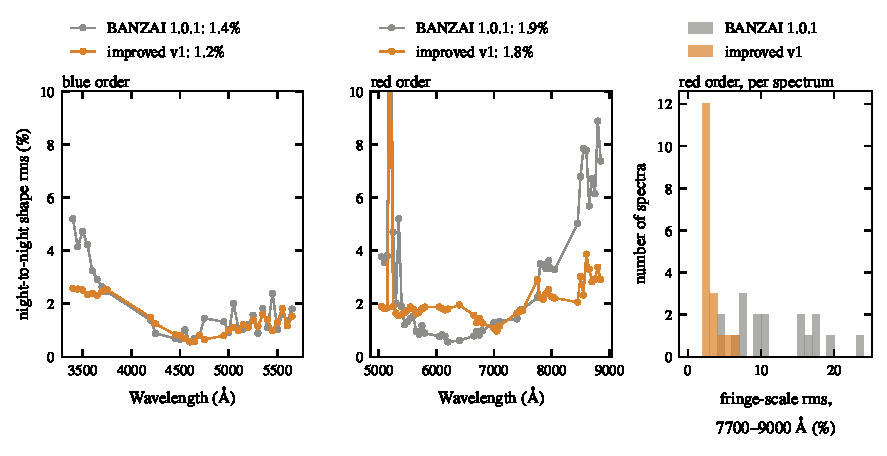
\includegraphics[width=\textwidth]{figures/fig_standard.pdf}
\caption{EG\,21 closure test. Left and middle: night-to-night rms of the shape of the 18 calibrated EG\,21 spectra
relative to the CTIO reference in its 50\,\AA{} bins (telluric and Balmer bins masked): archive (grey) and this work
(each night calibrated with the median sensitivity of the other 17 nights). Right: fringe-scale rms of the red order.}
\label{fig:standard}
\end{figure}


